
\documentclass[tikz,border=6pt]{standalone}
\usepackage{pgfplots}
\usepgfplotslibrary{groupplots}
\usetikzlibrary{arrows.meta,calc,positioning,backgrounds}
\pgfplotsset{compat=1.18}
\definecolor{ink}{HTML}{16324F}
\definecolor{rowc}{HTML}{1B4965}
\definecolor{colc}{HTML}{A44A3F}
\definecolor{accent}{HTML}{D9A441}
\definecolor{sage}{HTML}{4F6D5B}
\definecolor{sand}{HTML}{E7DFC6}
\definecolor{mist}{HTML}{F4F1EA}
\definecolor{gridc}{HTML}{D7D3C8}
\pagecolor{mist}
\begin{document}

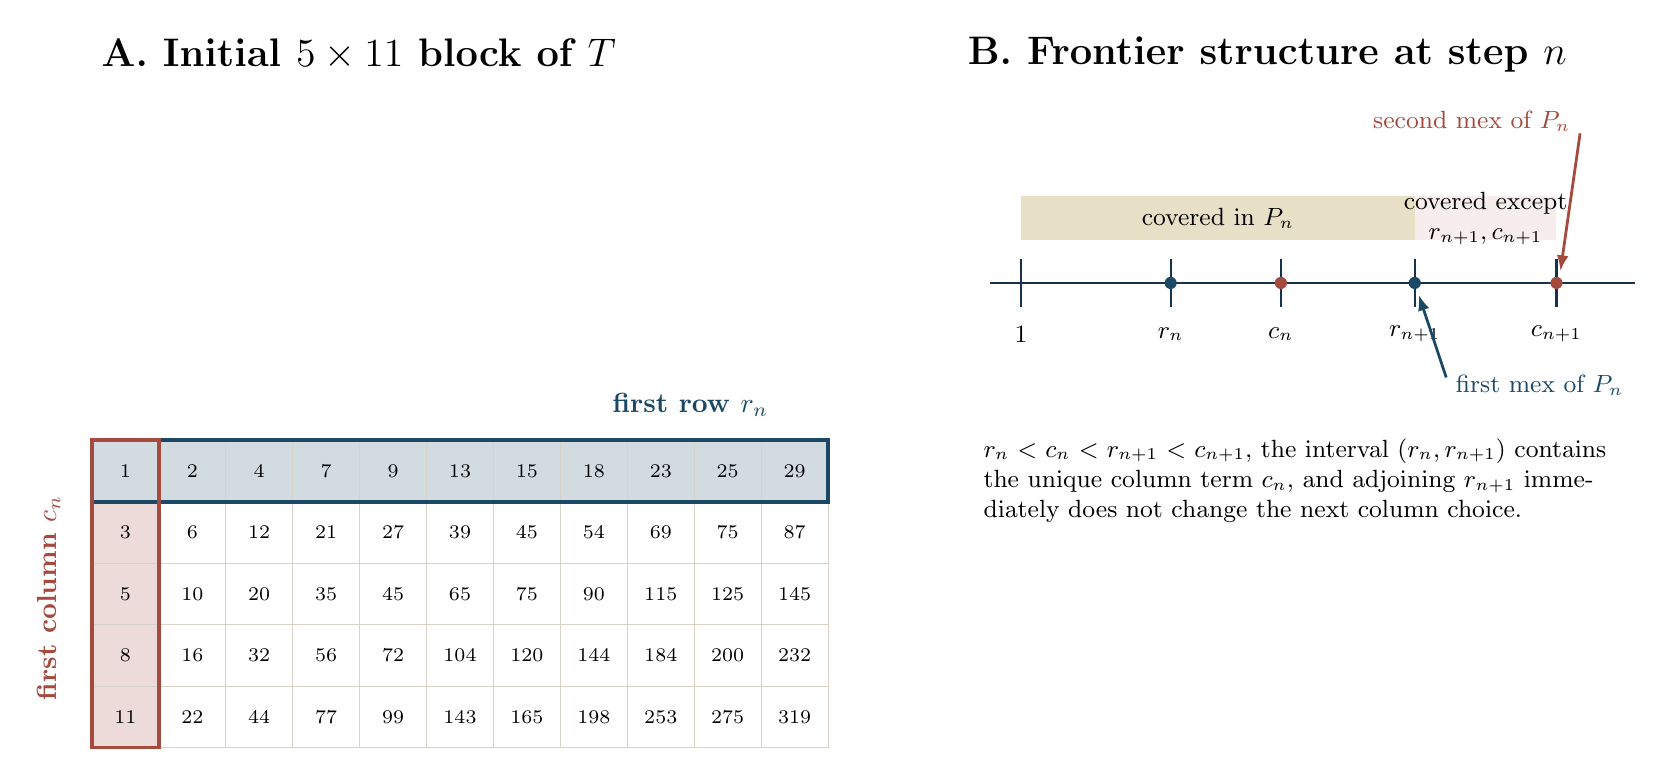
\begin{tikzpicture}[font=\small]
\node[font=\bfseries\Large, anchor=west] at (0,4.9) {A. Initial $5\times 11$ block of $T$};
\filldraw[fill=rowc!20, draw=gridc, line width=0.4pt] (0.000,0.000) rectangle (0.850,-0.780);
\node[font=\scriptsize] at (0.425,-0.390) {1};
\filldraw[fill=rowc!20, draw=gridc, line width=0.4pt] (0.850,0.000) rectangle (1.700,-0.780);
\node[font=\scriptsize] at (1.275,-0.390) {2};
\filldraw[fill=rowc!20, draw=gridc, line width=0.4pt] (1.700,0.000) rectangle (2.550,-0.780);
\node[font=\scriptsize] at (2.125,-0.390) {4};
\filldraw[fill=rowc!20, draw=gridc, line width=0.4pt] (2.550,0.000) rectangle (3.400,-0.780);
\node[font=\scriptsize] at (2.975,-0.390) {7};
\filldraw[fill=rowc!20, draw=gridc, line width=0.4pt] (3.400,0.000) rectangle (4.250,-0.780);
\node[font=\scriptsize] at (3.825,-0.390) {9};
\filldraw[fill=rowc!20, draw=gridc, line width=0.4pt] (4.250,0.000) rectangle (5.100,-0.780);
\node[font=\scriptsize] at (4.675,-0.390) {13};
\filldraw[fill=rowc!20, draw=gridc, line width=0.4pt] (5.100,0.000) rectangle (5.950,-0.780);
\node[font=\scriptsize] at (5.525,-0.390) {15};
\filldraw[fill=rowc!20, draw=gridc, line width=0.4pt] (5.950,0.000) rectangle (6.800,-0.780);
\node[font=\scriptsize] at (6.375,-0.390) {18};
\filldraw[fill=rowc!20, draw=gridc, line width=0.4pt] (6.800,0.000) rectangle (7.650,-0.780);
\node[font=\scriptsize] at (7.225,-0.390) {23};
\filldraw[fill=rowc!20, draw=gridc, line width=0.4pt] (7.650,0.000) rectangle (8.500,-0.780);
\node[font=\scriptsize] at (8.075,-0.390) {25};
\filldraw[fill=rowc!20, draw=gridc, line width=0.4pt] (8.500,0.000) rectangle (9.350,-0.780);
\node[font=\scriptsize] at (8.925,-0.390) {29};
\filldraw[fill=colc!20, draw=gridc, line width=0.4pt] (0.000,-0.780) rectangle (0.850,-1.560);
\node[font=\scriptsize] at (0.425,-1.170) {3};
\filldraw[fill=white, draw=gridc, line width=0.4pt] (0.850,-0.780) rectangle (1.700,-1.560);
\node[font=\scriptsize] at (1.275,-1.170) {6};
\filldraw[fill=white, draw=gridc, line width=0.4pt] (1.700,-0.780) rectangle (2.550,-1.560);
\node[font=\scriptsize] at (2.125,-1.170) {12};
\filldraw[fill=white, draw=gridc, line width=0.4pt] (2.550,-0.780) rectangle (3.400,-1.560);
\node[font=\scriptsize] at (2.975,-1.170) {21};
\filldraw[fill=white, draw=gridc, line width=0.4pt] (3.400,-0.780) rectangle (4.250,-1.560);
\node[font=\scriptsize] at (3.825,-1.170) {27};
\filldraw[fill=white, draw=gridc, line width=0.4pt] (4.250,-0.780) rectangle (5.100,-1.560);
\node[font=\scriptsize] at (4.675,-1.170) {39};
\filldraw[fill=white, draw=gridc, line width=0.4pt] (5.100,-0.780) rectangle (5.950,-1.560);
\node[font=\scriptsize] at (5.525,-1.170) {45};
\filldraw[fill=white, draw=gridc, line width=0.4pt] (5.950,-0.780) rectangle (6.800,-1.560);
\node[font=\scriptsize] at (6.375,-1.170) {54};
\filldraw[fill=white, draw=gridc, line width=0.4pt] (6.800,-0.780) rectangle (7.650,-1.560);
\node[font=\scriptsize] at (7.225,-1.170) {69};
\filldraw[fill=white, draw=gridc, line width=0.4pt] (7.650,-0.780) rectangle (8.500,-1.560);
\node[font=\scriptsize] at (8.075,-1.170) {75};
\filldraw[fill=white, draw=gridc, line width=0.4pt] (8.500,-0.780) rectangle (9.350,-1.560);
\node[font=\scriptsize] at (8.925,-1.170) {87};
\filldraw[fill=colc!20, draw=gridc, line width=0.4pt] (0.000,-1.560) rectangle (0.850,-2.340);
\node[font=\scriptsize] at (0.425,-1.950) {5};
\filldraw[fill=white, draw=gridc, line width=0.4pt] (0.850,-1.560) rectangle (1.700,-2.340);
\node[font=\scriptsize] at (1.275,-1.950) {10};
\filldraw[fill=white, draw=gridc, line width=0.4pt] (1.700,-1.560) rectangle (2.550,-2.340);
\node[font=\scriptsize] at (2.125,-1.950) {20};
\filldraw[fill=white, draw=gridc, line width=0.4pt] (2.550,-1.560) rectangle (3.400,-2.340);
\node[font=\scriptsize] at (2.975,-1.950) {35};
\filldraw[fill=white, draw=gridc, line width=0.4pt] (3.400,-1.560) rectangle (4.250,-2.340);
\node[font=\scriptsize] at (3.825,-1.950) {45};
\filldraw[fill=white, draw=gridc, line width=0.4pt] (4.250,-1.560) rectangle (5.100,-2.340);
\node[font=\scriptsize] at (4.675,-1.950) {65};
\filldraw[fill=white, draw=gridc, line width=0.4pt] (5.100,-1.560) rectangle (5.950,-2.340);
\node[font=\scriptsize] at (5.525,-1.950) {75};
\filldraw[fill=white, draw=gridc, line width=0.4pt] (5.950,-1.560) rectangle (6.800,-2.340);
\node[font=\scriptsize] at (6.375,-1.950) {90};
\filldraw[fill=white, draw=gridc, line width=0.4pt] (6.800,-1.560) rectangle (7.650,-2.340);
\node[font=\scriptsize] at (7.225,-1.950) {115};
\filldraw[fill=white, draw=gridc, line width=0.4pt] (7.650,-1.560) rectangle (8.500,-2.340);
\node[font=\scriptsize] at (8.075,-1.950) {125};
\filldraw[fill=white, draw=gridc, line width=0.4pt] (8.500,-1.560) rectangle (9.350,-2.340);
\node[font=\scriptsize] at (8.925,-1.950) {145};
\filldraw[fill=colc!20, draw=gridc, line width=0.4pt] (0.000,-2.340) rectangle (0.850,-3.120);
\node[font=\scriptsize] at (0.425,-2.730) {8};
\filldraw[fill=white, draw=gridc, line width=0.4pt] (0.850,-2.340) rectangle (1.700,-3.120);
\node[font=\scriptsize] at (1.275,-2.730) {16};
\filldraw[fill=white, draw=gridc, line width=0.4pt] (1.700,-2.340) rectangle (2.550,-3.120);
\node[font=\scriptsize] at (2.125,-2.730) {32};
\filldraw[fill=white, draw=gridc, line width=0.4pt] (2.550,-2.340) rectangle (3.400,-3.120);
\node[font=\scriptsize] at (2.975,-2.730) {56};
\filldraw[fill=white, draw=gridc, line width=0.4pt] (3.400,-2.340) rectangle (4.250,-3.120);
\node[font=\scriptsize] at (3.825,-2.730) {72};
\filldraw[fill=white, draw=gridc, line width=0.4pt] (4.250,-2.340) rectangle (5.100,-3.120);
\node[font=\scriptsize] at (4.675,-2.730) {104};
\filldraw[fill=white, draw=gridc, line width=0.4pt] (5.100,-2.340) rectangle (5.950,-3.120);
\node[font=\scriptsize] at (5.525,-2.730) {120};
\filldraw[fill=white, draw=gridc, line width=0.4pt] (5.950,-2.340) rectangle (6.800,-3.120);
\node[font=\scriptsize] at (6.375,-2.730) {144};
\filldraw[fill=white, draw=gridc, line width=0.4pt] (6.800,-2.340) rectangle (7.650,-3.120);
\node[font=\scriptsize] at (7.225,-2.730) {184};
\filldraw[fill=white, draw=gridc, line width=0.4pt] (7.650,-2.340) rectangle (8.500,-3.120);
\node[font=\scriptsize] at (8.075,-2.730) {200};
\filldraw[fill=white, draw=gridc, line width=0.4pt] (8.500,-2.340) rectangle (9.350,-3.120);
\node[font=\scriptsize] at (8.925,-2.730) {232};
\filldraw[fill=colc!20, draw=gridc, line width=0.4pt] (0.000,-3.120) rectangle (0.850,-3.900);
\node[font=\scriptsize] at (0.425,-3.510) {11};
\filldraw[fill=white, draw=gridc, line width=0.4pt] (0.850,-3.120) rectangle (1.700,-3.900);
\node[font=\scriptsize] at (1.275,-3.510) {22};
\filldraw[fill=white, draw=gridc, line width=0.4pt] (1.700,-3.120) rectangle (2.550,-3.900);
\node[font=\scriptsize] at (2.125,-3.510) {44};
\filldraw[fill=white, draw=gridc, line width=0.4pt] (2.550,-3.120) rectangle (3.400,-3.900);
\node[font=\scriptsize] at (2.975,-3.510) {77};
\filldraw[fill=white, draw=gridc, line width=0.4pt] (3.400,-3.120) rectangle (4.250,-3.900);
\node[font=\scriptsize] at (3.825,-3.510) {99};
\filldraw[fill=white, draw=gridc, line width=0.4pt] (4.250,-3.120) rectangle (5.100,-3.900);
\node[font=\scriptsize] at (4.675,-3.510) {143};
\filldraw[fill=white, draw=gridc, line width=0.4pt] (5.100,-3.120) rectangle (5.950,-3.900);
\node[font=\scriptsize] at (5.525,-3.510) {165};
\filldraw[fill=white, draw=gridc, line width=0.4pt] (5.950,-3.120) rectangle (6.800,-3.900);
\node[font=\scriptsize] at (6.375,-3.510) {198};
\filldraw[fill=white, draw=gridc, line width=0.4pt] (6.800,-3.120) rectangle (7.650,-3.900);
\node[font=\scriptsize] at (7.225,-3.510) {253};
\filldraw[fill=white, draw=gridc, line width=0.4pt] (7.650,-3.120) rectangle (8.500,-3.900);
\node[font=\scriptsize] at (8.075,-3.510) {275};
\filldraw[fill=white, draw=gridc, line width=0.4pt] (8.500,-3.120) rectangle (9.350,-3.900);
\node[font=\scriptsize] at (8.925,-3.510) {319};
\draw[rowc, line width=1.4pt] (0,0) rectangle (9.350,-0.780);
\draw[colc, line width=1.4pt] (0,0) rectangle (0.850,-3.900);
\node[rowc, font=\bfseries] at (7.6,0.45) {first row $r_n$};
\node[colc, font=\bfseries, rotate=90] at (-0.55,-2.0) {first column $c_n$};
\begin{scope}[xshift=11.0cm]
\node[font=\bfseries\Large, anchor=west] at (0,4.9) {B. Frontier structure at step $n$};
\draw[ink, line width=0.8pt] (0.4,2.0) -- (8.6,2.0);
\draw[ink, line width=0.8pt] (0.8,1.7) -- (0.8,2.3);
\node at (0.8,1.35) {$ 1 $};
\draw[ink, line width=0.8pt] (2.7,1.7) -- (2.7,2.3);
\node at (2.7,1.35) {$ r_n $};
\draw[ink, line width=0.8pt] (4.1,1.7) -- (4.1,2.3);
\node at (4.1,1.35) {$ c_n $};
\draw[ink, line width=0.8pt] (5.8,1.7) -- (5.8,2.3);
\node at (5.8,1.35) {$ r_{n+1} $};
\draw[ink, line width=0.8pt] (7.6,1.7) -- (7.6,2.3);
\node at (7.6,1.35) {$ c_{n+1} $};
\fill[sand] (0.8,2.55) rectangle (5.8,3.1);
\fill[colc!10] (5.8,2.55) rectangle (7.6,3.1);
\node at (3.3,2.82) {covered in $P_n$};
\node[align=center] at (6.7,2.82) {covered except\\$r_{n+1},c_{n+1}$};
\fill[rowc] (2.7,2.0) circle (2.2pt);
\fill[colc] (4.1,2.0) circle (2.2pt);
\fill[rowc] (5.8,2.0) circle (2.2pt);
\fill[colc] (7.6,2.0) circle (2.2pt);
\draw[-{Latex[length=2.0mm]}, rowc, line width=1.0pt] (6.2,0.8) -- (5.85,1.85);
\draw[-{Latex[length=2.0mm]}, colc, line width=1.0pt] (7.9,3.9) -- (7.65,2.15);
\node[rowc, anchor=west] at (6.2,0.7) {first mex of $P_n$};
\node[colc, anchor=east] at (7.9,4.05) {second mex of $P_n$};
\node[align=left, text width=8.0cm, anchor=north west] at (0.2,0.15) {$r_n<c_n<r_{n+1}<c_{n+1}$, the interval $(r_n,r_{n+1})$ contains the unique column term $c_n$, and adjoining $r_{n+1}$ immediately does not change the next column choice.};
\end{scope}
\end{tikzpicture}

\end{document}
